\section{Livello rete}
Mette in comunicazione \textit{logica} gli \textbf{host}. È implementato in ogni livello, sia nei \textit{router} che nei \textit{sistemi terminali}. È colui che trasporta i vari \textit{segmenti} (mandati dal livello di trasporto) e li \textit{incapsula} in \textbf{datagrammi} lato mittente, mentre il destinatario consegna i \textbf{datagrammi} al livello trasporto, quindi \textit{segmenti}.

Ci sono due funzioni principali a livello di rete
\begin{itemize}
  \item \textbf{Inoltro o forwarding}: è un'azione \textit{locale}, definisce qual è il percorso per il destinatario designato, dipende dall'\textbf{instradamento}, l'\textit{instradamento} \textit{informa} le decisioni di inoltro e aggiorna i percorsi e li comunica all'\textit{inoltro}.
  \item \textbf{Instradamento o routing}: Consiste nel trovare (non come) la strada migliore per andare da una sorgente a una destinazione. Gli algoritmi di instradamento determinano i \textit{percorsi} che i pacchetti seguono.
\end{itemize}

\subsection{Architettura del router}
Nel router abbiamo due componenti, una si occupa dell'instradamento, calcolando i \textit{percorsi}, e una si occupa dell'inoltro, muovendo i \textit{pacchetti} lungo quei percorsi. In alto abbiamo la componente che gestisce l'instradamento con un \textbf{algoritmo di instradamento}, sotto abbiamo la componente che gestisce l'inoltro, che avrà una tabella con tutte le informazioni mandate dalla componente di instradamento.

Il primo piano si chiama \textbf{piano di controllo}, responsabile della gestione delle \textit{tabelle di instradamento}.

Il secondo piano si chiama \textbf{piano dei dati}, responsabile dell'elaborazione dei pacchetti ad \textit{alta velocità}, diviso in:

\begin{itemize}
  \item \textbf{Porte di ingresso}: porte logiche, non sono le porte fisiche, è uno stream di dati \textit{socket}. Hanno il livello fisico (ricezione di dati), livello di collegamento (ethernet) e livello di rete con la commutazione decentralizzata: determina la porta d'uscita dei pacchetti tramite la tabella d'inoltro, nel caso in cui arrivano tanti datagrammi che il router non riesce a manipolare man mano crea un \textit{buffer di accodamento} dove memorizza i pacchetti. Le porte di ingresso eseguono la \textit{ricezione a livello fisico, l'elaborazione a livello di collegamento e la ricerca a livello di rete}.
  \item \textbf{Struttura di commutazione}: inizialmente era un computer che manipolava i dati e aveva le porte come periferiche (\textit{Commutazione in memoria}), un metodo \textit{più vecchio e più lento}, ora usiamo la \textbf{commutazione tramite bus}: le porte d'ingresso gestiscono l'indirizzamento del pacchetto, manipolano loro la circuiteria per l'instradamento, un metodo \textit{più efficiente}. La soluzione ideale è \textbf{crossbar switch}, sono percorsi in parallelo con $2n$ bus che collegano $n$ porte d'ingresso a $n$ porte d'uscita, una struttura di commutazione \textit{non bloccante}.
  \item \textbf{Porte di uscita}: porte logiche, non sono le porte fisiche, è uno stream di dati \textit{socket}. Hanno gli stessi livelli della \textit{porta d'ingresso} ma in modo speculare. Le porte di uscita eseguono l'\textit{elaborazione a livello di rete, l'elaborazione a livello di collegamento e la trasmissione a livello fisico}. Le funzionalità di \textit{livello rete} sono: \textbf{funzionalità di accodamento} che riframmenta i pacchetti nel caso in cui il \textit{livello di collegamento} ha un \textit{MTU} (Maximum Transmission Unit) inferiore al precedente. Le porte di uscita eseguono l'\textit{accodamento} e la \textit{frammentazione} quando necessario.
\end{itemize}

\subsubsection{Tabelle di inoltro}
Le tabelle di inoltro, utilizzate per determinare la porta di uscita di un pacchetto, sono elaborate e aggiornate dal processore di instradamento. Una copia di queste tabelle è memorizzata su ciascuna porta di ingresso per velocizzare il processo di inoltro.

\textbf{Ricerca del prefisso più lungo:}
\begin{itemize}
    \item La ricerca nella tabella di inoltro si basa sul confronto tra un prefisso dell'indirizzo di destinazione del pacchetto e le righe della tabella.
    \item Se un indirizzo di destinazione corrisponde a più righe, il router adotta la regola di corrispondenza a prefisso più lungo, inoltrando il pacchetto all'interfaccia di collegamento associata alla corrispondenza più lunga.
\end{itemize}

\textbf{Elaborazione alle porte di ingresso:}
\begin{itemize}
    \item La ricerca nella tabella di inoltro è effettuata in hardware.
    \item Oltre alla ricerca, le porte di ingresso eseguono anche:
        \begin{itemize}
            \item Elaborazione a livello fisico e di collegamento.
            \item Controllo e riscrittura del numero di versione del pacchetto, del checksum e del tempo di vita.
            \item Aggiornamento dei contatori per la gestione di rete.
        \end{itemize}
\end{itemize}

\textbf{Astrazione Match-Action:}
L'azione di cercare la corrispondenza tra l'indirizzo IP di destinazione e inviare il pacchetto alla porta di uscita specificata è un caso specifico di un'astrazione più generale "match-action", che viene eseguita in molti dispositivi di rete, non solo nei router.

\subsection{Protocollo internet: IP}
Il protocollo \textbf{IP} (sia in versione 4 che in versione 6) stabilisce:
\begin{itemize}
  \item Convenzioni di indirizzamento, ovvero come gli indirizzi IP sono usati per \textit{identificare univocamente} gli host sulla rete.
  \item Formato dei datagrammi, che include \textit{header fields} per il routing e il controllo.
  \item La manipolazione dei pacchetti, ovvero la \textit{frammentazione e il riassemblaggio} dei datagrammi.
\end{itemize}
Il protocollo IP fornisce un trasferimento di datagrammi \textit{non affidabile e connectionless}.
Il protocollo \textbf{ICMP}, dipendente dal protocollo \textit{IP}, ovvero i messaggi ICMP sono \textit{trasportati all'interno di datagrammi IP}:
\begin{itemize}
  \item Notifica gli errori, ovvero ICMP è usato per riportare \textit{errori di rete} come host irraggiungibili o timeout.
  \item Segnalazione del router, ovvero ICMP è usato per la \textit{scoperta dei router} e la \textit{scoperta del MTU del percorso}.
\end{itemize}

\subsection{IPv4, Protocollo IP versione 4}
Ogni \textit{interfaccia di host} e \textit{router} hanno un \textbf{indirizzo IP univoco da 32 bit}. 
L'\textbf{interfaccia} è il confine tra host e collegamento fisico, i \textit{router} devono avere almeno due collegamenti fisici  e per ogni \textit{interfaccia} è associato un \textbf{indirizzo IP}. 

\subsubsection{Formato dei datagrammi}
Lungo 32 bit. Abbiamo i seguenti campi:
\begin{enumerate}
  \item \begin{enumerate}
      \item \textbf{Versione} del protocollo (4 o 6)
      \item \textbf{Lunghezza intestazione}, variabile
      \item \textbf{Tipo di servizio} quanto è importante il datagramma (non molto utilizzato)
      \item \textbf{Lunghezza del datagramma}, che include sia l'header che i dati.
  \end{enumerate}
  \item \begin{enumerate}
      \item \textbf{Identificatore a 16 bit}: usato per il \textit{riassemblaggio} dei datagrammi frammentati.
      \item \textbf{flag}: usati per il \textit{controllo della frammentazione}.
      \item \textbf{Spiazzamento di frammentazione a 13bit}: indica la \textit{posizione del frammento} nel datagramma originale.
  \end{enumerate}
  \item \begin{enumerate}
      \item \textbf{Tempo di vita residuo}: \textit{TTL - Time to live}, quanti router può attraversare il datagramma, il datagramma nasce con un tempo di vita previsto, a ogni passaggio viene decrementato di 1, quando il \textit{TTL} arriva a 0 il router elimina il pacchetto. Il TTL è usato per \textit{prevenire i loop di instradamento}.
      \item \textbf{Protocollo di livello superiore}: specifica quale \textit{protocollo} stiamo utilizzando a livello di \textit{trasporto}, per sapere a quale servizio del \textit{sistema operativo} mandare i pacchetti. Questo campo indica il \textit{protocollo usato dal payload} (es. TCP o UDP).
      \item \textbf{Checksum} della sola intestazione, stesso algoritmo del protocollo \textit{UDP}, chiamato \textbf{checksum internet}, non comprende il campo \textit{Dati}. Viene calcolata da ogni \textit{router} in cui passa. Il checksum è calcolato solo sull'\textit{header} e non sui dati.
  \end{enumerate}
  \item \textbf{Indirizzo IP origine}
  \item \textbf{Indirzzo IP destinazione}
  \item \textbf{Campi opzionali}: usati per \textit{funzionalità opzionali} come la sicurezza o il timestamping.
  \item \textbf{Dati}
\end{enumerate}

\begin{center}
  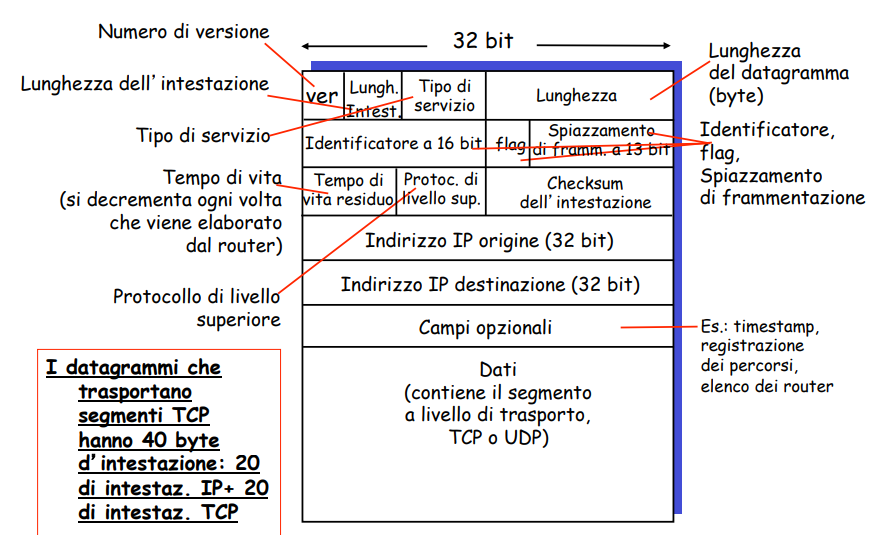
\includegraphics[width=\textwidth]{img/ipdatagramma.png}
\end{center}

\subsubsection{Frammentazione dei datagrammi IP}
L'unità massima di trasmissione (\textbf{MTU}) è la quantità massima di dati che possono passare in quel determinato \textit{livello di collegamento}. MTU è un concetto del \textit{livello di collegamento}.
I \textbf{datagrammi IP} vengono frammentati in \textit{datagrammi} \textit{più piccoli} quando un datagramma è \textit{più grande dell'MTU} di un collegamento.

\subsubsection{Sottorete}
L'\textit{indirizzo IP} è diviso in due parti, per l'\textit{indirizzamento gerarchico}:
\begin{itemize}
  \item \textbf{Parte di sottorete}: bit di alto ordine, che identificano la \textit{rete} o la \textit{sottorete}.
  \item \textbf{Parte dell'host}: bit di basso ordine, che identificano l'\textit{host specifico} all'interno della sottorete.
\end{itemize}
Una sottorete è definita anche come \textit{reti IP}, ovvero una \textit{rete logicamente separata} all'interno di una rete più grande.

\subsubsection{Assegnazione indirizzi internet CIDR}
\textbf{CIDR}: Classes InterDomain Routing, un \textit{metodo per allocare indirizzi IP} e \textit{instradare pacchetti IP}.
L'\textit{indirizzo IP} viene diviso in $a.b.c.d/x$ dove $x$ è un numero in bit che definisce la \textbf{maschera di rete}, ovvero il \textit{numero di bit nel prefisso di rete}.
Facendo $32 - x$ avremo il numero di bit \textit{"liberi"} per la \textit{sottorete}, ovvero il \textit{numero di bit disponibili per gli indirizzi host} nella sottorete.
\subsubsection*{Esempio}
$200.23.16.0/23$ diventa $11001000.000101111.0001000\textbf{0}.\textbf{00000000}$ dove la parte in grassetto è la \textbf{parte di host}, mentre il resto è il \textbf{prefisso di rete}. Avendo $x=23$ faremo $32-23 = 9$, quindi avremo correttamente $9$ bit di \textbf{parte di host}.

\subsubsection{Indirizzamento - convenzioni}
\begin{itemize}
  \item \textbf{Broadcast}: tutti i bit della \textbf{parte di host} posti a $1$. Il datagramma viene consegnato a \textit{tutti gli host} della sottorete.
  \item \textbf{Identificativo della rete}: Tutti i bit della \textbf{parte di host} è posta a $0$. Indirizzo della rete, usato per \textit{identificare la sottorete stessa}.
  \item \textbf{Identificatore del router}: solitamente il primo indirizzo disponibile (dopo quelli \textbf{riservati}, ovvero alcuni indirizzi sono \textit{riservati} e non possono essere usati per gli host) è del \textit{router}, usato come \textit{default gateway} per gli host nella sottorete.
\end{itemize}

\subsubsection{Netmask}
Una \textbf{netmask} è una sequenza di 32 bit associata a un indirizzo IP per l'individuazione del prefisso di rete e parte di host. La netmask è usata \textit{insieme a un indirizzo IP} per determinare la parte di rete e la parte host.
I bit che valgono $1$ identificano la \textit{parte di rete} e quelli che valgono $0$ identificano la \textit{parte di host}. La sequenza \textit{contigua} di 1 identifica la parte di rete e la sequenza \textit{contigua} di 0 identifica la parte host.
\begin{center}
  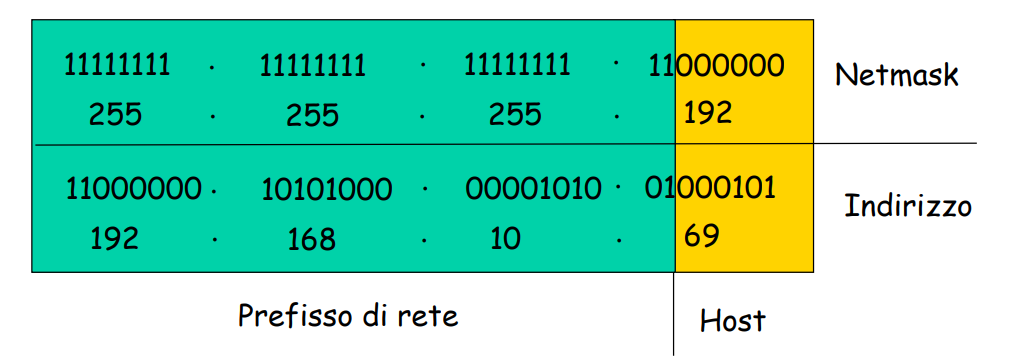
\includegraphics[width=\textwidth, height=3cm, keepaspectratio]{./img/netmask.png}
\end{center}
L'immagine mostra come la netmask separa la parte di rete e la parte host di un indirizzo IP.

\subsubsection{Inoltro dei pacchetti: Host}
Operazioni:
\begin{enumerate}
  \item Verifica se il destinatario è nella stessa sottorete: si effettua l'\textit{AND} tra il proprio indirizzo e la propria \textit{netmask}, e l'\textit{AND} tra l'indirizzo di destinazione e la propria \textit{netmask}, per \textit{estrarre il prefisso di rete} da entrambi gli indirizzi, e si verifica se sono uguali.
  \item Se è sulla stessa \textit{sottorete} invia direttamente all'host, usando l'\textit{indirizzo di livello collegamento} del destinatario. Se non è sulla stessa \textit{sottorete} invia al router, che è il \textit{default gateway} per la sottorete.
\end{enumerate}

\subsubsection{Inoltro dei pacchetti: Router}
Il router esegue le seguenti operazioni per inoltrare un pacchetto:
\begin{itemize}
  \item Verifica se il destinatario è in una delle sottoreti direttamente connesse al router.
  \item Altrimenti, per ogni riga della tabella di routing:
  \begin{itemize}
    \item Esegue un AND logico tra l'indirizzo di destinazione e la netmask della riga.
    \item Verifica se il risultato è uguale alla rete di destinazione.
  \end{itemize}
  \item Tra tutte le righe che hanno avuto successo, sceglie quella con la netmask più lunga.
  \item Se non c'è corrispondenza, invia sulla default route.
\end{itemize}

\subsubsection{Come ottenere un blocco di indirizzi IP}
Bisogna contattare il proprio \textbf{ISP} e ottenere la divisione in otto blocchi uguali di indirizzi contigui. Gli ISP sono responsabili di \textit{allocare gli indirizzi IP} ai loro clienti. La divisione in otto blocchi è una \textit{pratica comune} ma non un requisito rigido. Gli indirizzi contigui sono importanti per un \textit{instradamento efficiente}.

\subsubsection{Come ottenere un singolo indirizzo}
Due approcci:
\begin{itemize}
  \item \textbf{configurazione manuale}: si imposta manualmente l'indirizzo IP alla macchina, richiedendo l'\textit{intervento di un amministratore}.
  \item \textbf{DHCP}: Dynamic Host Configuration Protocol, un \textit{protocollo client-server}, assegna automaticamente un indirizzo IP, una subnet mask, un default gateway e altri parametri di rete una volta connesso in rete.
\end{itemize}

\subsubsection{DHCP}
È una funzionalità di livello rete ma gestita da un processo a livello applicativo che utilizza delle socket UDP, porta con numero 67 (il server usa la porta 67 come \textit{porta di destinazione}), mentre i client aprono la porta 68 (il client usa la porta 68 come \textit{porta di destinazione}) con indirizzo IP $0.0.0.0$. DHCP è un \textit{protocollo a livello applicativo} che usa UDP.

Il client appena inserito sulla rete non ha, giustamente, indirizzo IP e non conosce l'indirizzo IP del server DHCP, quindi il client invia un messaggio \textit{broadcast} (usando un \textit{indirizzo broadcast limitato} come 255.255.255.255) sulla porta 67, cercando un server DHCP, anche il server DHCP risponderà in \textit{broadcast} (usando un \textit{indirizzo broadcast limitato}), poiché il destinatario non ha ancora un \textit{indirizzo IP}.

Consente di ottenere \textbf{dinamicamente} gli indirizzi IP degli \textit{host}, assegnando indirizzi IP da un \textit{pool di indirizzi disponibili}. Non assegna obbligatoriamente lo stesso IP all'host, varia in base a quelli che ha disponibile. Il \textbf{transaction ID} serve al \textit{server} per sapere con chi sta parlando e a chi assegnare l'\textit{indirizzo IP}, usato per \textit{abbinare richieste e risposte}.
\begin{enumerate}
  \item \textbf{DHCP discover} da parte degli host, un messaggio broadcast a tutta la rete alla ricerca di un \textbf{server DHCP}.
  \item \textbf{DHCP offer}: il \textit{server DHCP} offre un indirizzo IP all'host.
  \item \textbf{DHCP request}: l'host accetta l'indirizzo IP proposto dal \textit{server DHCP}.
  \item \textbf{DHCP ack}: il \textit{server DHCP} invia l'ack di conferma.
\end{enumerate}

\subsubsection{NAT}
Consente di separare una rete specifica dalle altre, crea la \textbf{rete privata}. L'acronimo è: \textbf{Network address translation}, usato per \textit{conservare gli indirizzi IP pubblici}.

Il \textbf{NAT} si trova all'interno del \textit{router}, che si trova al \textit{confine} tra la rete privata e quella pubblica. Le reti esterne vedono la rete privata come un \textbf{unico} \textit{indirizzo IP}, che sarà quello assegnato al \textit{router}. L'indirizzo IP pubblico è l'\textit{unico indirizzo IP} visibile all'esterno. Le macchine all'interno della \textit{rete privata} avranno degli \textbf{indirizzi IP privati}, che saranno visibili solo all'interno della \textit{rete privata}. Le reti private usano \textit{range di indirizzi IP privati}.

Il vantaggio è di avere un unico indirizzo IP fornito dall'\textit{ISP} per la \textbf{rete pubblica}, andando a mascherare gli \textit{indirizzi IP privati} alle \textit{rete esterne}.

\subsubsection*{Implementazione}
Il router NAT riceve un datagramma, genera un numero di porta d'origine per quella macchina che ha mandato il datagramma, sostituisce l'indirizzo IP d'origine con il proprio per la rete esterna e sostituisce il numero di porta iniziale con quello generato precedentemente. Il router NAT \textit{mantiene una tabella di traduzione} per mappare indirizzi IP privati e porte a indirizzi IP pubblici e porte.

Il router accede al datagramma, modificando nell'\textit{header IP} e nell'\textit{header del livello di trasporto} la porta d'origine e ricalcola la checksum a livello trasporto, poi cambia l'indirizzo IP e ricalcola la checksum a livello di rete.

Il protocollo NAT può gestire al massimo tante connessioni quante sono le porte disponibili, quindi NAT ha \textit{limitazioni} nel numero di connessioni concorrenti.

\subsection{IPv6}
Il motivo per cui è stato progettato il protocollo \textbf{IP versione 6} è che si stanno esaurendo gli indirizzi IP a 32 bit. Gli indirizzi IPv6 sono \textit{128 bit}, rispetto ai 32 bit di IPv4. Inoltre è stato progettato per migliorare l'infrastruttura generale e velocizzarla.

\subsubsection{Formato dei datagrammi}
Il formato dei datagrammi \textbf{IPv6} ha un'intestazione a 40 byte ed è di lunghezza \textit{fissa} e \textit{semplificata} al contrario della versione 4. Inoltre non è consentita la frammentazione, il router non potrà frammentare il datagramma, la frammentazione è gestita dagli \textit{end system} in IPv6.
\begin{enumerate}
  \item
    \begin{enumerate}
      \item \textbf{ver}: versione del protocollo IP in uso.
      \item \textbf{pri}: priorità di flusso, indica la priorità del datagramma.
      \item \textbf{flow level}: identifica i datagrammi appartenenti allo stesso flusso.
    \end{enumerate}
  \item
    \begin{enumerate}
      \item \textbf{payload len}: lunghezza del payload del datagramma.
      \item \textbf{next hdr}: indica il tipo di header successivo (es. TCP, UDP, extension header).
      \item \textbf{hop limit}: ttl, indica il numero massimo di hop che il datagramma può attraversare.
    \end{enumerate}
  \item \textbf{source address}: indirizzo di origine a \textit{128 bit}.
  \item \textbf{destination address}: indirizzo di destinazione a \textit{128 bit}.
  \item \textbf{data}
\end{enumerate}
\begin{center}
  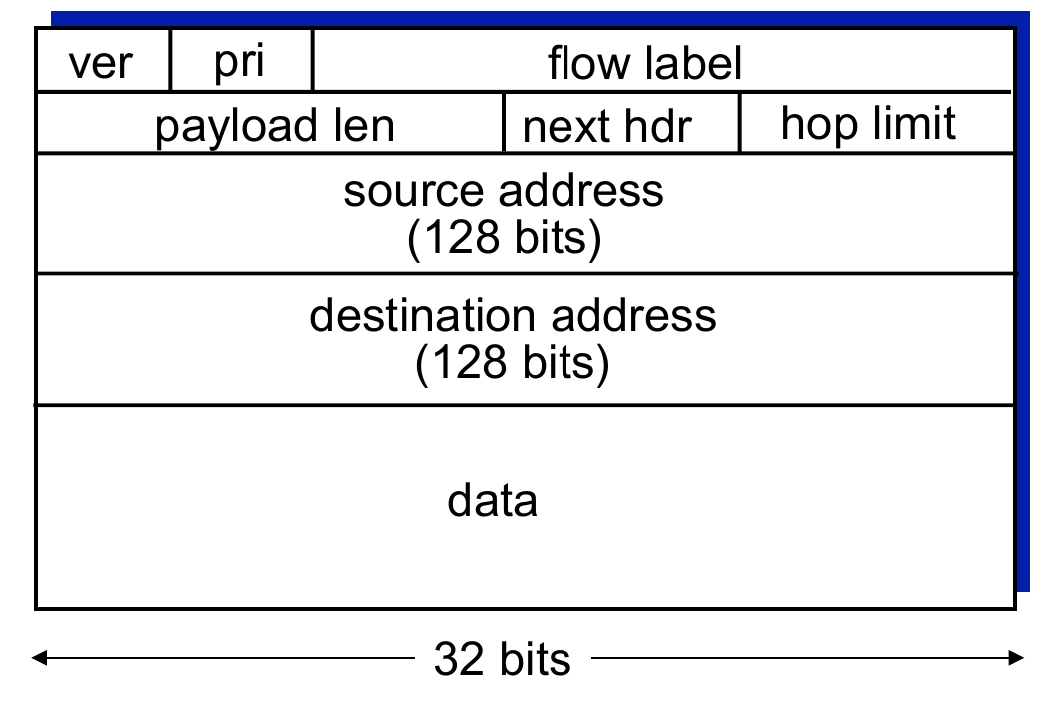
\includegraphics[width=\textwidth]{img/datagramma_ipv6.png}
\end{center}

Le varie novità di \textbf{IPv6} sono:
\begin{itemize}
  \item Elimina i campi di frammentazione.
  \item Checksum: eliminata dall'header IP e gestita dai livelli superiori.
  \item Opzioni: il campo non è scomparso ma è nelle \textit{extension headers} puntate da "next hdr".
  \item ICMPv6: nuova versione di ICMP, usata per la \textit{scoperta dei vicini} e la \textit{scoperta dei router}, oltre che per la segnalazione degli errori.
\end{itemize}
Il protocollo riesce a mascherare i datagrammi IPv6 in datagrammi IPv4 quando si passa su un hop che parla solo IPv4, tramite il tunneling che permette di \textit{incapsulare i datagrammi IPv6 in datagrammi IPv4}.
